\documentclass[tikz]{scrartcl}
\usepackage{scrhack}
\usepackage[british]{babel}		%Hypenation rules
\usepackage[T1]{fontenc}		%Font encoding
\usepackage[utf8]{inputenc}		%Input encoding

\usepackage[paperheight=58mm,paperwidth=88mm,margin=0mm]{geometry}


\usepackage{tgheros}
\usepackage{charter}
\usepackage[bitstream-charter]{mathdesign}
\normalfont
\usepackage{pifont} %For extra symbols
\usepackage{calligra}

\usepackage{tikz}
\usetikzlibrary{matrix}

\usepackage{xcolor,colortbl}

\definecolor{normal}{HTML}{A8A878}
\definecolor{figthing}{HTML}{C03028}
\definecolor{flying}{HTML}{A890F0}
\definecolor{poison}{HTML}{A040A0}
\definecolor{ground}{HTML}{E0C068}
\definecolor{rock}{HTML}{B8A038}
\definecolor{bug}{HTML}{A8B820}
\definecolor{ghost}{HTML}{705898}
\definecolor{steel}{HTML}{B8B8D0}
\definecolor{fire}{HTML}{F08030}
\definecolor{water}{HTML}{6890F0}
\definecolor{grass}{HTML}{78C850}
\definecolor{electric}{HTML}{F8D030}
\definecolor{psychic}{HTML}{F85888}
\definecolor{ice}{HTML}{98D8D8}
\definecolor{dragon}{HTML}{7038F8}
\definecolor{dark}{HTML}{705848}
\definecolor{fairy}{HTML}{EE99AC}

\definecolor{lines}{HTML}{EEEEEE}

\definecolor{eff}{HTML}{84FF84}
\definecolor{res}{HTML}{FF8484}
\definecolor{imm}{HTML}{A9A9A9}

\begin{document}
\begin{figure}
  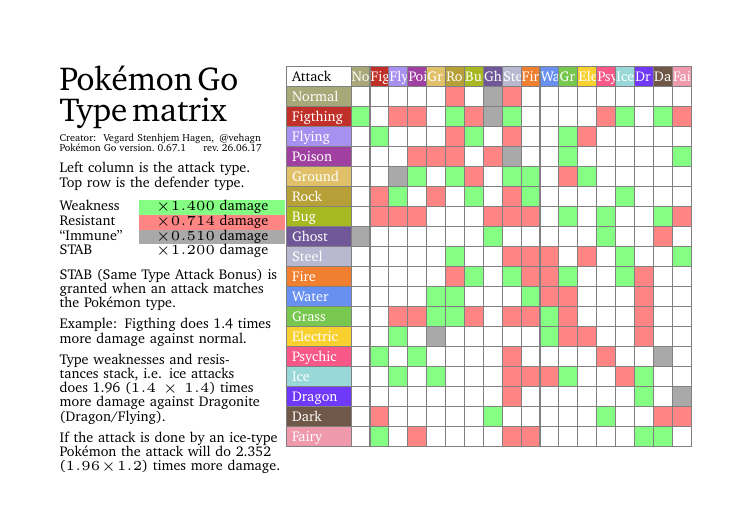
\begin{tikzpicture}[font=\fontsize{1.8mm}{1.8mm}\selectfont\strut]
  \begin{scope}[xshift=14.5mm]
    \matrix[matrix of nodes, 
            nodes={draw=gray,minimum size=2.2mm,inner sep=.1mm,outer sep=0,anchor=center,text width=2.2mm,align=left,text height=1.8mm,text=white},
            nodes in empty cells,
            column sep=-\pgflinewidth,
            row sep=-\pgflinewidth]{
 |[text=black,text width=8mm]|~Attack $\blacktriangleright$              & |[fill=normal]|  No   &  |[fill=figthing]| Fig & |[fill=flying]|  Fly  &   |[fill=poison]| Poi  &   |[fill=ground]| Gr  & |[fill=rock]| Ro & |[fill=bug]| Bu & |[fill=ghost]| Gh & |[fill=steel]| Ste & |[fill=fire]| Fir & |[fill=water]| Wa & |[fill=grass]| Gr & |[fill=electric]| Ele & |[fill=psychic]| Psy & |[fill=ice]| Ice & |[fill=dragon ]| Dr & |[fill=dark]| Da & |[fill=fairy]| Fai \\
|[fill=normal,text width=8mm]|   ~Normal   &            &            &            &            &            &|[fill=res]|&            &|[fill=imm]|&|[fill=res]|&            &            &            &            &            &            &            &            &            \\
|[fill=figthing,text width=8mm]| ~Figthing &|[fill=eff]|&            &|[fill=res]|&|[fill=res]|&            &|[fill=eff]|&|[fill=res]|&|[fill=imm]|&|[fill=eff]|&            &            &            &            &|[fill=res]|&|[fill=eff]|&            &|[fill=eff]|&|[fill=res]|\\
|[fill=flying,text width=8mm]|   ~Flying   &            &|[fill=eff]|&            &            &            &|[fill=res]|&|[fill=eff]|&            &|[fill=res]|&            &            &|[fill=eff]|&|[fill=res]|&            &            &            &            &            \\
|[fill=poison,text width=8mm]|   ~Poison   &            &            &            &|[fill=res]|&|[fill=res]|&|[fill=res]|&            &|[fill=res]|&|[fill=imm]|&            &            &|[fill=eff]|&            &            &            &            &            &|[fill=eff]|\\
|[fill=ground,text width=8mm]|   ~Ground   &            &            &|[fill=imm]|&|[fill=eff]|&            &|[fill=eff]|&|[fill=res]|&            &|[fill=eff]|&|[fill=eff]|&            &|[fill=res]|&|[fill=eff]|&            &            &            &            &            \\
|[fill=rock,text width=8mm]|     ~Rock     &            &|[fill=res]|&|[fill=eff]|&            &|[fill=res]|&            &|[fill=eff]|&            &|[fill=res]|&|[fill=eff]|&            &            &            &            &|[fill=eff]|&            &            &            \\
|[fill=bug,text width=8mm]|      ~Bug      &            &|[fill=res]|&|[fill=res]|&|[fill=res]|&            &            &            &|[fill=res]|&|[fill=res]|&|[fill=res]|&            &|[fill=eff]|&            &|[fill=eff]|&            &            &|[fill=eff]|&|[fill=res]|\\
|[fill=ghost,text width=8mm]|    ~Ghost    &|[fill=imm]|&            &            &            &            &            &            &|[fill=eff]|&            &            &            &            &            &|[fill=eff]|&            &            &|[fill=res]|&            \\
|[fill=steel,text width=8mm]|    ~Steel    &            &            &            &            &            &|[fill=eff]|&            &            &|[fill=res]|&|[fill=res]|&|[fill=res]|&            &|[fill=res]|&            &|[fill=eff]|&            &            &|[fill=eff]|\\
|[fill=fire,text width=8mm]|     ~Fire     &            &            &            &            &            &|[fill=res]|&|[fill=eff]|&            &|[fill=eff]|&|[fill=res]|&|[fill=res]|&|[fill=eff]|&            &            &|[fill=eff]|&|[fill=res]|&            &            \\
|[fill=water,text width=8mm]|    ~Water    &            &            &            &            &|[fill=eff]|&|[fill=eff]|&            &            &            &|[fill=eff]|&|[fill=res]|&|[fill=res]|&            &            &            &|[fill=res]|&            &            \\
|[fill=grass,text width=8mm]|    ~Grass    &            &            &|[fill=res]|&|[fill=res]|&|[fill=eff]|&|[fill=eff]|&|[fill=res]|&            &|[fill=res]|&|[fill=res]|&|[fill=eff]|&|[fill=res]|&            &            &            &|[fill=res]|&            &            \\
|[fill=electric,text width=8mm]| ~Electric &            &            &|[fill=eff]|&            &|[fill=imm]|&            &            &            &            &            &|[fill=eff]|&|[fill=res]|&|[fill=res]|&            &            &|[fill=res]|&            &            \\
|[fill=psychic,text width=8mm]|  ~Psychic  &            &|[fill=eff]|&            &|[fill=eff]|&            &            &            &            &|[fill=res]|&            &            &            &            &|[fill=res]|&            &            &|[fill=imm]|&            \\
|[fill=ice,text width=8mm]|      ~Ice      &            &            &|[fill=eff]|&            &|[fill=eff]|&            &            &            &|[fill=res]|&|[fill=res]|&|[fill=res]|&|[fill=eff]|&            &            &|[fill=res]|&|[fill=eff]|&            &            \\
|[fill=dragon,text width=8mm]|   ~Dragon   &            &            &            &            &            &            &            &            &|[fill=res]|&            &            &            &            &            &            &|[fill=eff]|&            &|[fill=imm]|\\
|[fill=dark,text width=8mm]|     ~Dark     &            &|[fill=res]|&            &            &            &            &            &|[fill=eff]|&            &            &            &            &            &|[fill=eff]|&            &            &|[fill=res]|&|[fill=res]|\\
|[fill=fairy,text width=8mm]|    ~Fairy    &            &|[fill=eff]|&            &|[fill=res]|&            &            &            &            &|[fill=res]|&|[fill=res]|&            &            &            &            &            &|[fill=eff]|&|[fill=eff]|&            \\
    };
    \end{scope}
    \draw[opacity=0] (-44mm,-29mm) rectangle (44mm,29mm);
    \node[align=left,anchor=north,text width=28mm] at (-26mm,25.5mm) {
        {\large Pokémon Go \\ Type matrix} \\
            \vspace{.2em}        
            {\fontsize{1.3mm}{1.3mm}\selectfont
            Creator: {Vegard\hspace{.3em}Stenhjem\hspace{.3em}Hagen}, @vehagn \\
            Pokémon\hspace{.3em}Go\hspace{.3em}version.\hspace{.3em}0.67.1 \hspace{.75em} rev.\hspace{.3em}26.06.17\\}
            \vspace{.5em}
            Left column is the attack type.\\
            Top row is the defender type.\\
            \vspace{.5em}
            \begin{tabular}{@{}l  l}
                Weakness  & \cellcolor{eff}$\times 1.400$ damage\\
                Resistant & \cellcolor{res}$\times 0.714$ damage\\
                ``Immune''    & \cellcolor{imm}$\times 0.510$ damage\\
                STAB & $\times 1.200$ damage
            \end{tabular}\\
            \vspace{.5em}
            STAB (Same Type Attack Bonus) is granted when an attack matches \\ the Pokémon type.\\
            \vspace{.5em}                   
            Example: Figthing does 1.4 times more damage against normal.\\
            \vspace{.5em}
            Type weaknesses and resistances stack, i.e. ice attacks does 1.96 ($1.4 \times 1.4$) times more damage against {Dragonite} (Dragon/Flying).\\
            \vspace{.5em}
            If the attack is done by an ice-type Pokémon the attack will do 2.352 ($1.96 \times 1.2$) times more damage.
    };
  \end{tikzpicture}
\end{figure}
\end{document}